\documentclass[12pt,a4paper,utf8x]{report}

% Pour pouvoir utiliser 
\usepackage{ucs}
\usepackage[utf8x]{inputenc}

\usepackage{url} % Pour avoir de belles url
\usepackage {geometry}

% Pour mettre du code source
\usepackage {listings}
% Pour pouvoir passer en paysage
\usepackage{lscape}

% Pour pouvoir faire plusieurs colonnes
\usepackage {multicol}
% Pour crééer un index
\usepackage{makeidx}
\makeindex

% Pour gérer les liens interractifs et les signets Acrobat
\usepackage{hyperref}
\hypersetup{
pdftitle={titre de mon document},
pdfauthor={Nom de l'auteur},
pdfsubject={Sujet du document},
pdfkeywords={les mots clefs},
bookmarks, % Création du signet
pdfstartview=FitH, % Page de la largeur de la fenêtre
colorlinks=true, % Liens en couleur
linkcolor=black, 	
anchorcolor=black, 	
citecolor=black, 	
filecolor=black, 	
menucolor=black,
runcolor=black,
urlcolor=black, 	
frenchlinks=black,
bookmarksnumbered=true, % Signet numéroté
pdfpagemode=UseOutlines, % Montre les bookmarks.
bookmarksopen =true,
}

% Pour afficher la bibliographie, mais pas nottoc (Table of Contents), notlof (List of Figures) ni notlot (List of Tables)
\usepackage[notlof, notlot]{tocbibind}


% Pour les entetes de page
% \usepackage{fancyheadings}
%\pagestyle{fancy}
%\renewcommand{\sectionmark}[1]{\markboth{#1}{}} 
%\renewcommand{\subsectionmark}[1]{\markright{#1}} 

% Pour l'interligne de 1.5
\usepackage {setspace}
% Pour les marges de la page
\geometry{a4paper, top=2.5cm, bottom=3.5cm, left=1.5cm, right=1.5cm, marginparwidth=1.2cm}

\parskip=5pt %% distance entre § (paragraphe)
\sloppy %% respecter toujours la marge de droite 

% Pour les pénalités :
\interfootnotelinepenalty=150 %note de bas de page
\widowpenalty=150 %% veuves et orphelines
\clubpenalty=150 

%Pour la longueur de l'indentation des paragraphes
\setlength{\parindent}{15mm}



%%%% debut macro pour enlever le nom chapitre %%%%
\makeatletter
\def\@makechapterhead#1{%
  \vspace*{50\p@}%
  {\parindent \z@ \raggedright \normalfont
    \interlinepenalty\@M
    \ifnum \c@secnumdepth >\m@ne
        \Huge\bfseries \thechapter\quad
    \fi
    \Huge \bfseries #1\par\nobreak
    \vskip 40\p@
  }}

\def\@makeschapterhead#1{%
  \vspace*{50\p@}%
  {\parindent \z@ \raggedright
    \normalfont
    \interlinepenalty\@M
    \Huge \bfseries  #1\par\nobreak
    \vskip 40\p@
  }}
\makeatother
%%%% fin macro %%%%
 
\title
{
	\normalsize{
	University of Nantes\\
	2009-2010}\\
	\vspace{15mm}
	\Huge{Atari Go}
}
\author{Alexandre GARNIER \and Yann TREGUER \\
	\vspace{45mm}
}
 
\begin{document}

	\maketitle

	\tableofcontents
	
	\clearpage
	
	\begin{onehalfspace}

    \chapter{Introduction}
    
	This report will give you some kind of presentation of our Atari Go project, especially technical aspects, like global architecture or implementation of most important methods.
	
	But let us first introduce this wonderful game which is Atari Go.
	
	Atari go is a game derived from the famous chinese millenar strategy game : go. In go, stones - white or black depending on player - are freely placed on a plate named goban.
	
	Basically, the goal is to define zones. At the end of the game, player with the greatest zones win.
	
	In addition, a player can take other player's stones by taking all the liberties of this stone. The liberty of a stone is a free adjacent intersection.
	
	In atari go, the goal is only to be the first to take one stone.
	
	\clearpage
	
	\chapter{Class Diagrams}
	
	\section{Global architecture}
	
	Here is a first abstract diagram of our project, base on MVC pattern.
	
	\begin{figure}[h!]
		\centering
		\scalebox{1}{
			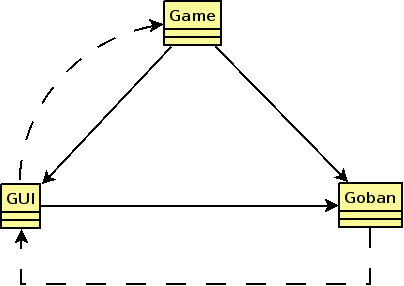
\includegraphics{images/global}
		}
		\caption{MVC}
		\label{mvc} 
	\end{figure}
	Game is the controler.
	
	GUI is the view.
	
	Goban is the model.
	
	\clearpage
	
	\section{Goban}
	
	\begin{figure}[h!]
		\centering
		\scalebox{0.8}{
			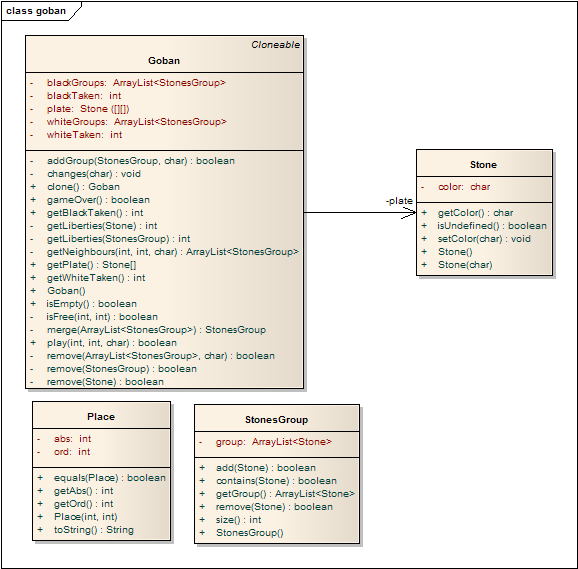
\includegraphics{images/goban}
		}
		\caption{Goban}
		\label{gbn} 
	\end{figure}
	
	A goban is characterized by a nine by nine grid.
	
	In order to guarantee the taken of stones, we also stock groups of stones of each colors in the Goban class attributes.
	
	\clearpage
	
	\section{Heuristics}
	
	\begin{figure}[h!]
		\centering
		\scalebox{0.8}{
			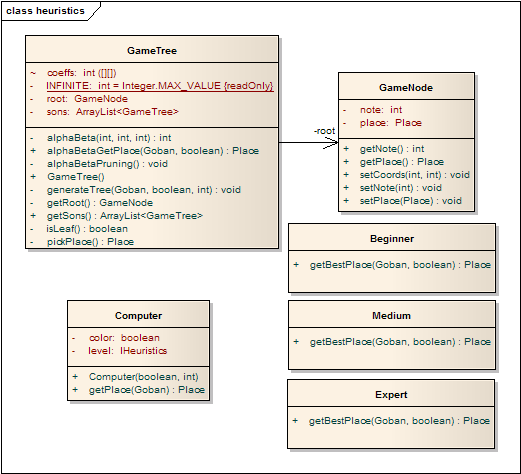
\includegraphics{images/heuristics}
		}
		\caption{Heuristics}
		\label{hrst} 
	\end{figure}
	
	The heuristics mainly allows to calculate the best place to play for the AI.
	
	Heuristics is applied by using Alpha-Beta pruning on a game tree which developps each possible place for each player on a setted depth.
	
	\clearpage
	
	\section{Graphic User Interface}
	
	\begin{figure}[h!]
		\centering
		\scalebox{0.8}{
			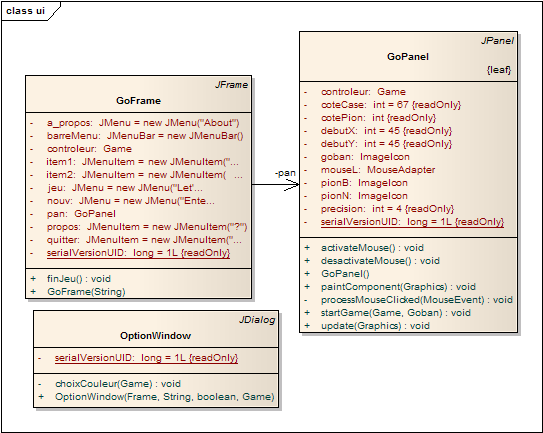
\includegraphics{images/ui}
		}
		\caption{GUI}
		\label{gui} 
	\end{figure}
	
	The GUI typically use two classes GoFrame and GoPanel, which extends respectively JFrame and JPanel, to provide the user a common Java graphic interface.
	
	\clearpage
	
	\section{Main program}
	
	\begin{figure}[h!]
		\centering
		\scalebox{0.8}{
			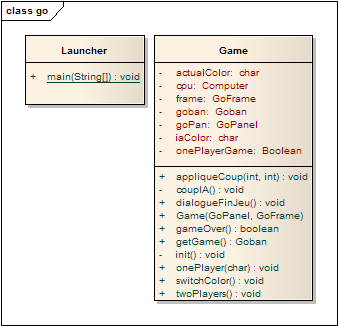
\includegraphics{images/go}
		}
		\caption{Main}
		\label{main} 
	\end{figure}
	
	Here we can see the details of the controler class, which link all the other packages to allow the application to run.
	
	\clearpage
	
	\chapter{The goban}
	
	The goban, described in class Goban from package fr.alma.go.goban, is characterized by a  9x9 stones' grid.

	Stones are characterized by their color, white, black or undefined (reflecting a empty intersection on the plate).
	
	Moreover, as we saw before, we also stock stones groups of each color in two different lists.

	For that, we implement a class StonesGroup which is in charge to stock all the stones of a group.

	Basically, this implies the followed facts :

	\begin{itemize}
		\item On each place played, the program checks the groups list of the place color, and stock each adjacent group to the stone in a temporary list. After that, all these groups are merged into one, and the stone is added to this new group. Finally, the program check if the group allways get at least one liberty.
		\item Just before the suicide check, the program checks the other color groups list, in order to see if one of them has lost all its liberties, and in this case the game is over, the last player has won.
	\end{itemize}

	\clearpage
	
	\chapter{The heuristics}
	
	Concerning the heuristics, in MVC pattern it takes place in Model, just like the goban.
	
	Globally, we have a Computer class, representing the AI player, which is in charge to link the Game controler to decision of the next place played.
	
	The heuristics chosen here is the alpha-beta pruning of a game tree :
	
	\begin{lstlisting}
	
	
function alphabeta(node, depth, alpha, beta)         
    if  depth = 0 "or" node is a terminal node
        return the heuristic value of node
    foreach child of node
        alpha := max(alpha, -alphabeta(child, depth-1, -beta, -alpha))     
      		(* use symmetry, -beta becomes subsequently pruned alpha *)
        if beta<=alpha
            break                             (* Beta cut-off *)
    return alpha

(* Initial call *)
alphabeta(origin, depth, -infinity, +infinity)
	\end{lstlisting}
	
	\clearpage
	
	\chapter{Conclusion}
	
	To get more technical informations on this project, we invite you to read its Javadoc.
	
	\end{onehalfspace}
 
\end{document}
